% ============================================================
%  Manual do Usuário — aneb-sim v0.9 (M9 / pré-release)
%  Compilar com: tectonic manual.tex
%  Saída:        manual.pdf
% ============================================================
\documentclass[12pt,a4paper]{article}

% --- Codificação e língua ----------------------------------------
\usepackage[utf8]{inputenc}
\usepackage[T1]{fontenc}
\usepackage[brazil]{babel}

% --- Tipografia --------------------------------------------------
\usepackage{lmodern}
\usepackage{microtype}

% --- Layout ------------------------------------------------------
\usepackage[
  top=2.5cm, bottom=2.5cm,
  left=2.8cm, right=2.8cm,
  headheight=15pt
]{geometry}
\usepackage{fancyhdr}
\usepackage{titlesec}
\usepackage{parskip}
\setlength{\parindent}{0pt}
\setlength{\parskip}{6pt}
\usepackage{enumitem}

% --- Cor e links (paleta verde-PCB do aneb-sim) ------------------
\usepackage{xcolor}
\definecolor{verdeescuro}{RGB}{15, 64, 40}
\definecolor{verdemedio}{RGB}{40, 120, 70}
\definecolor{verdeclaro}{RGB}{220, 245, 220}
\definecolor{cinzatexto}{RGB}{80, 80, 80}
\definecolor{amarelodest}{RGB}{255, 243, 205}
\definecolor{amarelob}{RGB}{180, 130, 0}
\definecolor{azuldest}{RGB}{220, 235, 250}
\definecolor{azulb}{RGB}{40, 100, 180}
\definecolor{vermelhodest}{RGB}{255, 220, 220}
\definecolor{vermelhob}{RGB}{160, 40, 40}

\usepackage[
  colorlinks=true,
  linkcolor=verdemedio,
  urlcolor=verdemedio,
  citecolor=verdemedio
]{hyperref}

% --- Tabelas -----------------------------------------------------
\usepackage{booktabs}
\usepackage{array}
\usepackage{colortbl}

% --- Caixas (notas, dicas, alertas) ------------------------------
\usepackage{tcolorbox}
\tcbuselibrary{skins,breakable}

\newtcolorbox{notabox}[1][Nota]{
  colback=amarelodest, colframe=amarelob,
  fonttitle=\bfseries\small, title=#1,
  left=4pt, right=4pt, top=3pt, bottom=3pt,
  breakable
}

\newtcolorbox{dicabox}[1][Dica]{
  colback=verdeclaro, colframe=verdemedio,
  fonttitle=\bfseries\small, title=#1,
  left=4pt, right=4pt, top=3pt, bottom=3pt,
  breakable
}

\newtcolorbox{alertabox}[1][Atenção]{
  colback=vermelhodest, colframe=vermelhob,
  fonttitle=\bfseries\small, title=#1,
  left=4pt, right=4pt, top=3pt, bottom=3pt,
  breakable
}

\newtcolorbox{infobox}[1][Informação]{
  colback=azuldest, colframe=azulb,
  fonttitle=\bfseries\small, title=#1,
  left=4pt, right=4pt, top=3pt, bottom=3pt,
  breakable
}

% --- Figuras -----------------------------------------------------
\usepackage{graphicx}
\graphicspath{{images/}}
\usepackage{float}

% --- Código ------------------------------------------------------
\usepackage{listings}
\lstset{
  basicstyle=\ttfamily\footnotesize,
  keywordstyle=\color{verdemedio}\bfseries,
  commentstyle=\color{gray},
  stringstyle=\color{verdemedio},
  backgroundcolor=\color{gray!8},
  frame=single,
  framerule=0.4pt,
  rulecolor=\color{gray!40},
  breaklines=true,
  showstringspaces=false,
  tabsize=2
}

% --- Cabeçalho e rodapé ------------------------------------------
\pagestyle{fancy}
\fancyhf{}
\fancyhead[L]{\small\color{cinzatexto}aneb-sim v0.9}
\fancyhead[R]{\small\color{cinzatexto}Manual do Usuário}
\fancyfoot[C]{\small\color{cinzatexto}\thepage}
\renewcommand{\headrulewidth}{0.4pt}
\renewcommand{\headrule}{\hbox to\headwidth{\color{verdemedio}\leaders\hrule height \headrulewidth\hfill}}

% --- Títulos de seção --------------------------------------------
\titleformat{\section}
  {\Large\bfseries\color{verdeescuro}}
  {\thesection.}{0.6em}{}
  [\color{verdemedio}\rule{\linewidth}{1.2pt}]

\titleformat{\subsection}
  {\large\bfseries\color{verdemedio}}
  {\thesubsection}{0.6em}{}

\titleformat{\subsubsection}
  {\normalsize\bfseries\color{verdemedio}}
  {\thesubsubsection}{0.6em}{}

% ================================================================
\begin{document}

% --- Capa --------------------------------------------------------
\begin{titlepage}
  \pagecolor{verdeescuro}
  \color{white}
  \vspace*{2cm}

  \begin{center}
    {\fontsize{11}{13}\selectfont\scshape Residência Tecnológica --- UFPE/CIn}\\[0.8cm]
    \rule{\linewidth}{1.5pt}\\[0.6cm]
    {\fontsize{28}{34}\selectfont\bfseries aneb-sim}\\[0.4cm]
    \rule{\linewidth}{1.5pt}\\[0.8cm]
    {\fontsize{15}{18}\selectfont Simulador da placa ANEB v1.1}\\[0.3cm]
    {\fontsize{12}{15}\selectfont\color{verdeclaro}%
      Sistemas Operacionais de Tempo Real --- Manual do Usuário}\\[2.5cm]
  \end{center}

  \begin{tcolorbox}[
    colback=white, colframe=white,
    coltext=verdeescuro,
    width=0.75\textwidth,
    center, arc=3pt,
    left=10pt, right=10pt, top=6pt, bottom=6pt
  ]
    \small
    \begin{tabular}{@{}ll@{}}
      \textbf{Versão}          & 0.9 (M9 / pré-release) \\
      \textbf{Data}            & Maio de 2026 \\
      \textbf{Repositório}     & \texttt{renatosfagundes/aneb-sim} \\
      \textbf{Plataforma}      & Windows 10/11 (MSYS2 + Python 3.11) \\
    \end{tabular}
  \end{tcolorbox}

  \vfill
  {\small\itshape Gerado por \texttt{docs/manual/manual.tex} --- Compilado com Tectonic}
\end{titlepage}
\pagecolor{white}
\color{black}

% --- Sumário -----------------------------------------------------
\tableofcontents
\newpage

% =================================================================
% 1. Introdução
% =================================================================
\section{Introdução}

O \textbf{aneb-sim} é um simulador de instruções da placa
\textbf{Automotive Network Evaluation Board v1.1} (ANEB) usada na
disciplina de Sistemas Operacionais de Tempo Real do CIn/UFPE.
Reproduz, em um único processo no PC do aluno, o comportamento dos
cinco microcontroladores da placa real:

\begin{itemize}[nosep]
  \item \textbf{ECU1}-\textbf{ECU4}: quatro ATmega328P, cada uma
        ligada a um controlador CAN MCP2515, dois LEDs digitais
        (DOUT0/DOUT1), quatro entradas analógicas com
        potenciômetros virtuais (AIN0--AIN3), quatro botões de
        entrada digital (DIN1--DIN4), um buzzer e um LCD I\textsuperscript{2}C
        16$\times$2;
  \item \textbf{MCU}: um ATmega328PB que roda o firmware de controle
        da placa (\texttt{MCU\_Firmware\_v08.hex}) e expõe os
        seletores de modo;
  \item \textbf{Barramento CAN1}: rede compartilhada entre as quatro
        ECUs, modelada com fidelidade de bit-stuffing, contadores
        TEC/REC e estados \emph{active} / \emph{passive} / \emph{bus-off};
\end{itemize}

\subsection{Por que um simulador?}

\begin{itemize}[nosep]
  \item \textbf{Acessibilidade}: não exige a placa física nem
        conexão VPN ao laboratório.
  \item \textbf{Reprodutibilidade}: o mesmo \texttt{.hex} compilado
        para a placa real roda no simulador --- não há porte de
        código.
  \item \textbf{Ferramentas}: o aluno usa \texttt{avrdude}, monitores
        seriais, e até o \emph{Remote Firmware Flasher} apontados
        para o simulador exatamente como apontariam para uma placa.
  \item \textbf{Diagnóstico}: estados internos (TEC/REC, free-RAM,
        sinais de barramento) ficam visíveis em tempo real, o que
        é difícil de obter em hardware.
\end{itemize}

\subsection{Funcionalidades}

\begin{itemize}[nosep]
  \item Engine em C com \texttt{simavr} (cinco núcleos AVR em paralelo,
        passo de \emph{lockstep} determinístico);
  \item Modelo MCP2515 fiel a nível de registrador (filtros, EFLG,
        bus-off, recuperação);
  \item Interface PyQt6/QML com painel por chip --- ilustração do
        Arduino Nano, LCD, LEDs domeados, potenciômetros angulares,
        botões DIN coloridos;
  \item Console serial por chip com texto colorido, contador de bytes,
        LED de atividade RX e \emph{follow}-toggle;
  \item Plotter por chip com até 14 sinais simultâneos (ADC, PWM,
        digitais), janela temporal selecionável e \emph{pause/resume};
  \item Painel de gravação \texttt{avrdude} com log colorizado e
        indicador de status (\emph{idle/flashing/success/done});
  \item \textbf{Optiboot embutido}: todo chip nasce com bootloader
        pré-carregado, então qualquer ferramenta (avrdude,
        Arduino IDE, Remote Flasher) consegue gravar firmware sem
        passos manuais;
  \item \textbf{Servidor TCP UART duplo}: porta de \emph{flasher}
        (\texttt{8600+i}) para gravação STK500 + porta de
        \emph{bridge} (\texttt{8700+i}) para encaminhamento passivo
        via portas COM virtuais (com0com);
  \item Integração com o \textbf{Remote Firmware Flasher} v2.4.0+
        como entrada \texttt{Localhost (aneb-sim)}.
\end{itemize}

% =================================================================
% 2. Instalação
% =================================================================
\section{Instalação}

\subsection{Pré-requisitos}

\begin{enumerate}[nosep]
  \item \textbf{Windows 10 ou 11} (64 bits).
  \item \textbf{MSYS2} com a toolchain \texttt{mingw-w64} --- veja
        \texttt{BOOTSTRAP.md} no repositório para passos detalhados.
  \item \textbf{Python 3.11.x} de
        \url{https://www.python.org/downloads/release/python-3112/}
        (não use 3.12 ou superior; o pacote \texttt{PyQt6} usado
        pela UI ainda fixa 3.11 nas suas roads).
  \item \textbf{Git} (qualquer versão recente).
\end{enumerate}

\subsection{Clone e bootstrap}

\begin{lstlisting}[language=bash]
git clone --recurse-submodules \
    https://github.com/renatosfagundes/aneb-sim.git /c/dev/aneb-sim
cd /c/dev/aneb-sim
./scripts/bootstrap.sh
\end{lstlisting}

O script \texttt{bootstrap.sh}:

\begin{itemize}[nosep]
  \item instala dependências do MSYS2 (\texttt{ninja},
        \texttt{cmake}, \texttt{libelf-dev}, etc.);
  \item compila o submódulo \texttt{simavr};
  \item cria o \texttt{venv} Python em \texttt{.venv/} e instala
        \texttt{PyQt6}, \texttt{pyserial} e similares.
\end{itemize}

\subsection{Primeira compilação}

\begin{lstlisting}[language=bash]
./scripts/build.sh
\end{lstlisting}

O \emph{output} é \texttt{build/aneb-sim/aneb-sim.exe}. Esse é o
\emph{engine} (binário C); a UI é Python e roda do mesmo
\texttt{venv}.

\subsection{Configuração das portas COM virtuais (com0com)}

Para que ferramentas externas (Remote Flasher, monitores seriais,
\texttt{avrdude} pela linha de comando) enxerguem cada chip do
simulador como uma porta COM, é necessário instalar pares
\texttt{com0com} virtuais.

\begin{lstlisting}[language=bash]
# Como administrador (PowerShell elevado ou cmd "Run as Admin")
scripts\setup_com.bat
\end{lstlisting}

O script:

\begin{enumerate}[nosep]
  \item instala o driver assinado da redistribuição do
        \emph{Pete Batard} (em \texttt{scripts\textbackslash com0com\_signed/});
  \item cria cinco pares de portas COM virtuais e os marca no
        registro do Windows com \texttt{FriendlyName}
        \texttt{ECU1 (aneb-sim)}, \texttt{ECU2 (aneb-sim)}, …,
        \texttt{MCU (aneb-sim)};
  \item escolhe automaticamente nomes COM livres
        (tipicamente \texttt{COM10}/\texttt{COM11},
        \texttt{COM12}/\texttt{COM13}, …).
\end{enumerate}

A UI do aneb-sim e o Remote Flasher leem o registro para descobrir
qual porta COM corresponde a cada chip --- não há configuração
manual.

\begin{notabox}[Removendo as portas]
  Para desinstalar os pares e o driver:
  \begin{lstlisting}[language=bash]
  scripts\remove_com.bat
  \end{lstlisting}
  Pode ser útil ao trocar de máquina, atualizar o Windows ou
  liberar números COM para outros usos.
\end{notabox}

% =================================================================
% 3. Primeira execução
% =================================================================
\section{Primeira execução}

\begin{lstlisting}[language=bash]
./scripts/run-ui.sh
\end{lstlisting}

A janela principal abre com o layout completo da placa: as quatro
ECUs em \emph{grid} 2$\times$2 à esquerda e o painel MCU à direita.
A barra superior mostra o título \textbf{ANEB v1.1} junto a botões
de controle (\textbf{Load}, \textbf{Pause}, \textbf{Resume},
\textbf{Speed}, \textbf{1$\times$}, \textbf{Max}, \textbf{Dashboard})
e ao indicador de \emph{engine} (\emph{running} em verde).

\begin{figure}[H]
  \centering
  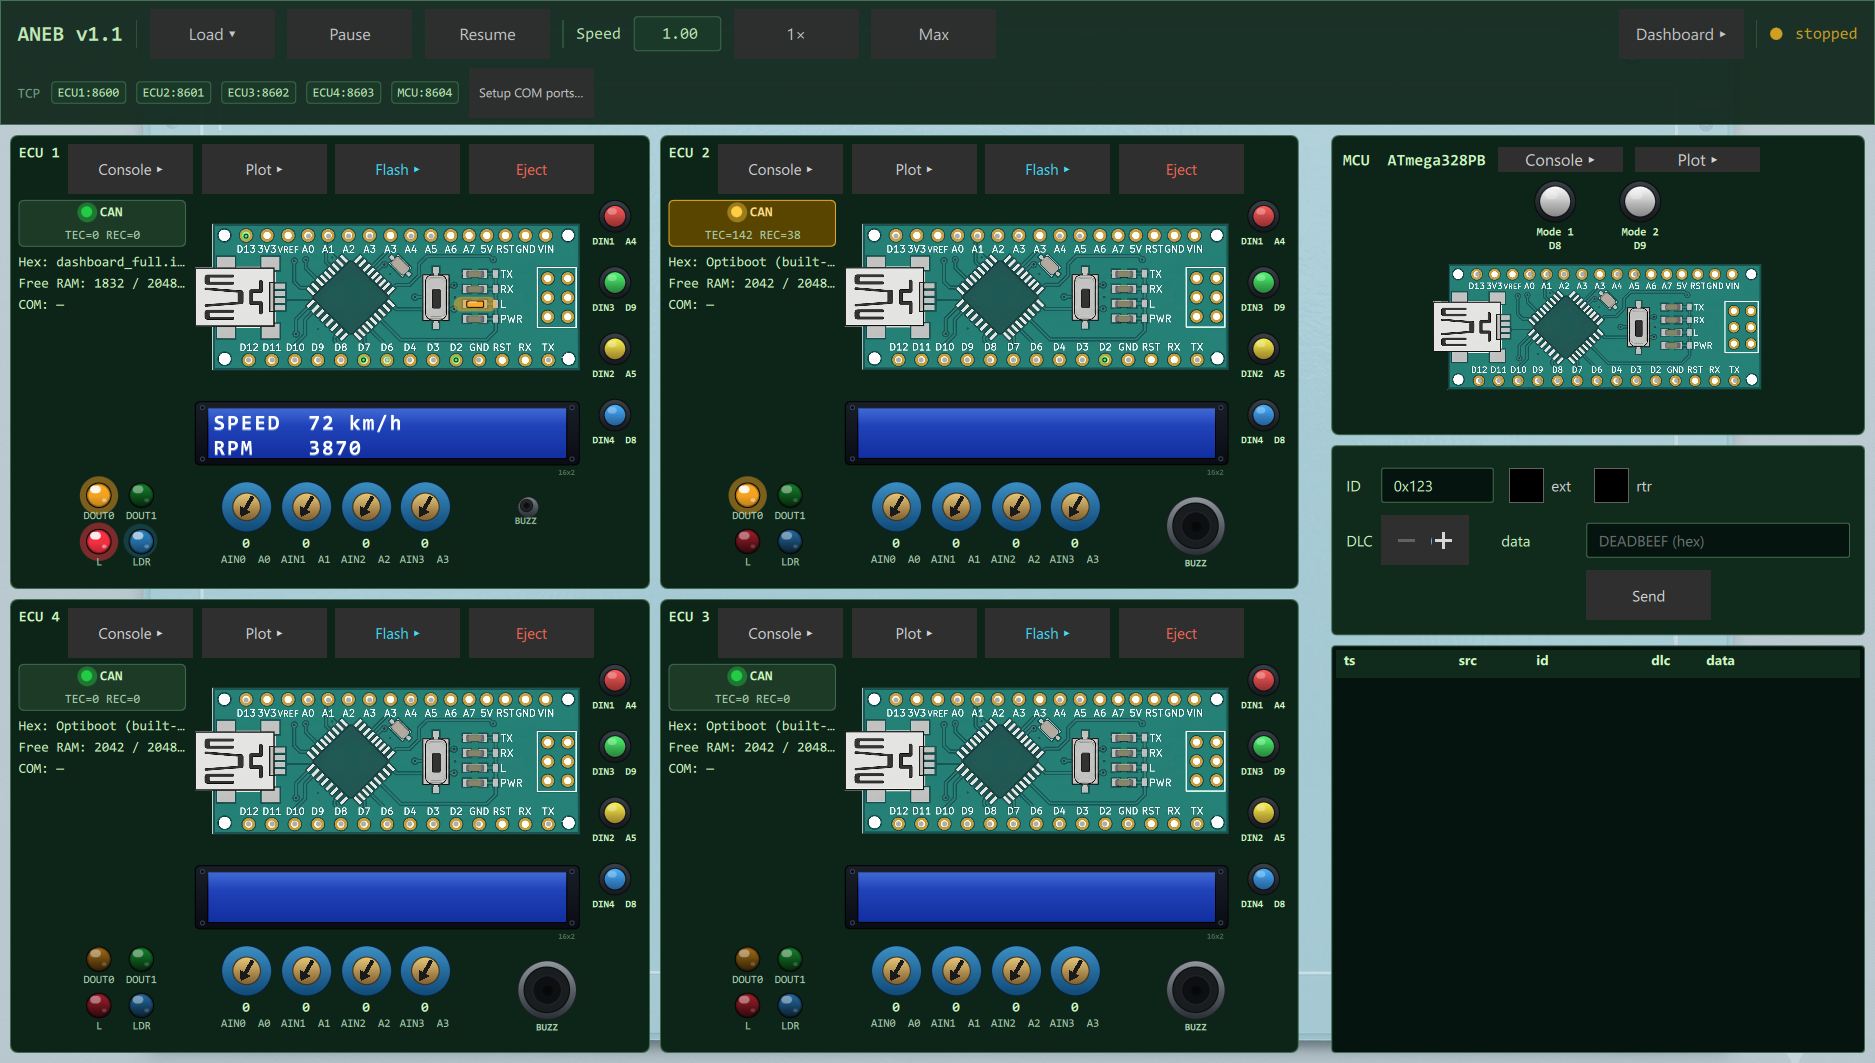
\includegraphics[width=\textwidth]{board_main.png}
  \caption{Janela principal do aneb-sim com as quatro ECUs e o MCU.
           Cada \emph{card} mostra a barra lateral com o status CAN e
           os metadados do firmware (Hex, Free RAM, COM), a ilustração
           do Arduino Nano e o LCD.}
\end{figure}

\subsection{O que acontece ao iniciar}

\begin{enumerate}[nosep]
  \item O \emph{engine} (\texttt{aneb-sim.exe}) é lançado como
        subprocesso da UI; sua \emph{stdout} JSON-Lines alimenta
        as bindings QML, e a \emph{stdin} recebe comandos da UI.
  \item Cada chip ATmega328P recebe automaticamente o
        \textbf{Optiboot} pré-carregado em \emph{flash} ---
        nasce pronto para receber comandos STK500.
  \item A \emph{bridge} interna conecta as cinco portas TCP UART
        (\texttt{8700+i}) às portas COM virtuais
        (\texttt{COM10}--\texttt{COM18}, lado bridge) e expõe a
        contraparte (\texttt{COM11}--\texttt{COM19}) para o usuário.
  \item Sem firmware do usuário, cada ECU executa um \emph{stub}
        \texttt{rjmp .self} --- ou seja, fica em \emph{idle} sem
        gerar tráfego. As janelas de Console, Plotter e Flash
        permanecem fechadas.
\end{enumerate}

% =================================================================
% 4. Visão geral da interface
% =================================================================
\section{Visão geral da interface}

\subsection{Painel ECU}

Cada uma das quatro ECUs ocupa um \emph{card} com a seguinte
disposição:

\begin{itemize}[nosep]
  \item \textbf{Linha de título} (topo): rótulo (\texttt{ECU 1},
        \texttt{ECU 2}, …) e três botões para abrir/fechar as
        janelas auxiliares: \textbf{Console}, \textbf{Plot} e
        \textbf{Flash}, mais um botão \textbf{Eject} para descarregar
        o firmware.
  \item \textbf{Barra lateral} (esquerda): pílula CAN com indicador
        de estado e contadores TEC/REC; abaixo dela, três linhas de
        metadados:
        \begin{itemize}[nosep]
          \item \texttt{Hex:}, com o nome do firmware atualmente
                em \emph{flash} (\texttt{Optiboot (built-in)} ao
                iniciar, ou o nome do \texttt{.hex} carregado);
          \item \texttt{Free RAM:}, com o valor estimado de SRAM
                livre (em bytes / total) calculado a partir do SP
                atual do chip;
          \item \texttt{COM:}, com a porta COM virtual da \emph{bridge}
                que o usuário deve abrir para ler/escrever a UART.
        \end{itemize}
        Passar o mouse sobre qualquer linha mostra um \emph{tooltip}
        com a explicação detalhada do valor.
  \item \textbf{Centro}: ilustração SVG do Arduino Nano com pinagem
        rotulada (\texttt{D0}--\texttt{D13}, \texttt{A0}--\texttt{A7})
        e LEDs internos (\texttt{TX}, \texttt{RX}, \texttt{L},
        \texttt{PWR}). Logo abaixo, o LCD I\textsuperscript{2}C 16$\times$2.
  \item \textbf{Botões DIN} (direita): quatro \emph{push-buttons}
        coloridos --- vermelho (DIN1/A4), verde (DIN3/D9), amarelo
        (DIN2/A5) e azul (DIN4/D8). Clicar simula o pressionamento
        físico do botão na placa real.
  \item \textbf{LEDs e potenciômetros} (rodapé): \texttt{DOUT0} e
        \texttt{DOUT1} (LEDs digitais), \texttt{L} (LED na placa),
        \texttt{LDR} (LED associado ao laço óptico), os quatro
        \emph{trim-pots} angulares para \texttt{AIN0}--\texttt{AIN3}
        e o \texttt{BUZZ} (representação do buzzer).
\end{itemize}

\subsection{Painel MCU}

À direita, o painel \textbf{MCU} mostra o ATmega328PB. Como o MCU
não está conectado ao barramento CAN nem aos periféricos das ECUs,
seu \emph{card} é mais enxuto: ilustração do Nano, LCD, e dois
seletores de \emph{modo} (\texttt{Mode 1} D8 / \texttt{Mode 2} D9).

\subsection{Toolbar}

\begin{itemize}[nosep]
  \item \textbf{Load \textbf{▾}}: menu de carregamento rápido que
        navega para \texttt{firmware/examples/} ou
        \texttt{firmware/mcu/} dependendo do contexto;
  \item \textbf{Pause}/\textbf{Resume}: pausam/retomam todos os chips
        de uma vez (útil para inspecionar estado);
  \item \textbf{Speed} (\texttt{0.5$\times$} / \texttt{1$\times$} /
        \texttt{Max}): multiplicador de \emph{wallclock}.
        \texttt{1$\times$} é tempo real (16 MHz), \texttt{Max} libera
        a simulação para correr o mais rápido que o PC permitir
        (útil para acelerar testes longos);
  \item \textbf{Dashboard}: abre uma janela compacta com a leitura
        ao vivo de todas as ECUs.
\end{itemize}

% =================================================================
% 5. Console serial
% =================================================================
\section{Console serial}

Cada ECU e o MCU têm uma janela de console serial dedicada,
acessível pelo botão \textbf{Console \textbf{\textgreater{}}} no painel do chip.
A janela mostra a saída UART do firmware em execução e permite
enviar caracteres de volta ao chip.

\begin{figure}[H]
  \centering
  
\includegraphics[width=0.85\textwidth]{ecu1_console.png}
  \caption{Janela de console serial mostrando saída UART de um sketch
           Plotter Arduino. Cabeçalho com chip badge, contador de bytes,
           LED de atividade RX, botão \emph{Clear} e \emph{toggle}
           \emph{Follow}; rodapé com campo de envio.}
\end{figure}

\subsection{Cabeçalho}

Da esquerda para a direita: emblema do chip (\texttt{ECU 1}), ponto
acentuado em ciano com o título \textbf{Console}, contador de bytes
recebidos, ponto verde que pisca a cada chunk de UART e três
controles de canto: \textbf{Clear} (apaga o buffer visível) e
\textbf{Follow} (\emph{auto-scroll} para a última linha). O
\emph{tooltip} no \textbf{Follow} explica o comportamento.

\subsection{Limites de buffer}

O console retém até 200\,000 caracteres em memória; ao ultrapassar
esse limite mais 50\,000 de \emph{slack}, o trecho mais antigo é
removido em uma operação só. Isso evita o consumo descontrolado de
memória quando um sketch \emph{Plotter} envia $\approx$11~KB/s
sem parar.

\begin{notabox}[Por que não retemos tudo?]
Reter o histórico inteiro fazia o slot \texttt{update\_uart} virar
$O(n^2)$: cada concatenação de \texttt{str + str} reconstrói a
string toda. Em alguns segundos a UI chegava a megabytes e a thread
do Qt travava por completo. O \emph{cap} mantém a janela de tempo
útil para depuração ($\approx$17~s a 11~KB/s) sem o custo
quadrático.
\end{notabox}

\subsection{Envio para o chip}

A barra inferior tem um campo de texto e o botão \textbf{Send}.
Pressionar \texttt{Enter} dispara o mesmo comportamento. O texto
digitado é enviado para o RX da UART do chip, com um \texttt{\textbackslash n}
adicionado ao final --- a maioria dos sketches usa
\texttt{Serial.readStringUntil('\textbackslash n')} ou similar.

% =================================================================
% 6. Plotter
% =================================================================
\section{Plotter}

O Plotter é uma janela com uma área de gráfico em \emph{rolling
window} mostrando até 14 sinais simultâneos do chip selecionado.
Acessível pelo botão \textbf{Plot \textbf{\textgreater{}}}.

\begin{figure}[H]
  \centering
  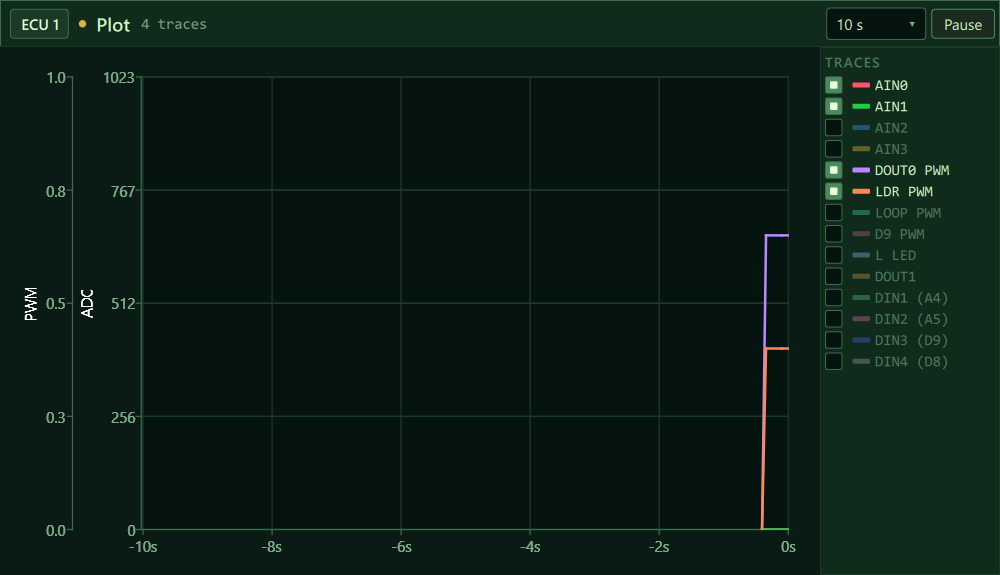
\includegraphics[width=\textwidth]{ecu1_plotter.png}
  \caption{Plotter com legenda dos 14 sinais disponíveis. Eixo Y
           esquerdo (0--1023) para ADCs, eixo Y direito (0,0--1,0)
           para canais PWM. Janela temporal selecionável (10\,s neste
           caso) e botão \emph{Pause} no canto superior direito.}
\end{figure}

\subsection{Cabeçalho}

\begin{itemize}[nosep]
  \item \textbf{Window} (\texttt{10\,s} / \texttt{30\,s} /
        \texttt{1\,min} / \texttt{5\,min}): seletor da janela
        temporal visível no eixo X. O eixo é ``segundos antes de
        agora''; \texttt{x = 0} é o instante atual.
  \item \textbf{Pause}/\textbf{Resume}: congela o gráfico mantendo
        a coleta de amostras; ao retomar, todos os pontos coletados
        durante a pausa aparecem.
\end{itemize}

\subsection{Catálogo de sinais}

A coluna direita lista todos os sinais expostos pelo bridge:

\begin{itemize}[nosep]
  \item \texttt{adc:0}--\texttt{adc:7}: leituras analógicas
        (eixo Y esquerdo, escala 0--1023);
  \item \texttt{pwm:PD3}, \texttt{pwm:PD5}, \texttt{pwm:PD6},
        \texttt{pwm:PB1}: \emph{duty cycles} dos canais PWM
        (eixo Y direito, escala 0,0--1,0);
  \item Mais traços digitais conforme o engine os exponha.
\end{itemize}

Cada \emph{checkbox} liga/desliga um traço; o \emph{swatch} de cor
escurece quando o traço está desligado.

\subsection{Amostragem}

O bridge da UI amostra a cada $\approx$50~ms (20~Hz) o estado de
cada sinal e mantém um \emph{ring buffer} de 6\,000 amostras por
sinal. Para janelas de 5~minutos, isso dá $\approx$20 amostras/s ---
suficiente para detectar variações de PWM com frequência $\leq$10~Hz
sem agredir o GPU.

% =================================================================
% 7. Gravação de firmware
% =================================================================
\section{Gravação de firmware}

\subsection{Pelo botão Flash da UI}

O fluxo nativo do aneb-sim usa o botão \textbf{Flash \textbf{\textgreater{}}}
em cada painel ECU. Ele abre a janela do \texttt{avrdude}
embutido, carrega o Optiboot empacotado no \emph{engine} e dispara
\texttt{avrdude -c arduino} via TCP em \texttt{net:127.0.0.1:8600+i}
(porta de \emph{flasher}).

\begin{figure}[H]
  \centering
  
\includegraphics[width=0.85\textwidth]{ecu1_avrdude.png}
  \caption{Janela do \texttt{avrdude} com log colorizado: linhas
           informativas em ciano, \emph{Writing}/\emph{Reading} com
           barra de progresso, \emph{verified}/\emph{Avrdude.EXE done}
           em verde indicando sucesso. O cabeçalho mostra o status
           atual (\emph{Success}) e três ações
           (\emph{Flash again} / \emph{Copy} / \emph{Clear}).}
\end{figure}

O cabeçalho mostra o status atual (\emph{Idle} / \emph{Flashing\dots} /
\emph{Success} / \emph{Done}) com cor correspondente, um ponto
pulsante enquanto a gravação está em curso, e três ações:
\textbf{Flash again}, \textbf{Copy} (copia o log inteiro para o
clipboard) e \textbf{Clear}.

\subsection{Externamente (Remote Flasher, Arduino IDE, linha de comando)}

Como o engine deixa o Optiboot pré-carregado em todos os chips, o
mesmo \texttt{.hex} pode ser gravado por qualquer ferramenta
\texttt{avrdude}-compatível que aceite o transporte
\texttt{net:host:port}:

\begin{lstlisting}[language=bash]
avrdude -c arduino -p atmega328p -b 115200 \
        -P net:127.0.0.1:8600 \
        -U flash:w:meu_sketch.ino.hex:i
\end{lstlisting}

A porta \texttt{8600+i} (\emph{flasher port}) tem semântica
DTR-pulse: cada \texttt{connect} dispara um reset interno do chip,
e o \texttt{disconnect} dispara um \emph{soft reset} (MCUSR=0) que
faz Optiboot pular direto para o sketch recém-gravado. O usuário
não precisa mexer em nenhum botão de \emph{reset}.

\begin{notabox}[Bridge da UI vs.\ flasher]
A bridge interna do aneb-sim usa a porta \emph{passiva}
\texttt{8700+i}; ela é expulsa automaticamente quando um
\texttt{avrdude} chega na porta \texttt{8600+i}. Após $\approx$5~s
do final da gravação, a bridge se reconecta sozinha e a saída UART
do firmware volta a fluir para a porta COM virtual --- não há
configuração nem botão para apertar.
\end{notabox}

% =================================================================
% 8. Integração com o Remote Firmware Flasher
% =================================================================
\section{Integração com o Remote Firmware Flasher}

A partir da versão 2.4.0, o \textbf{Remote Firmware Flasher}
detecta automaticamente o aneb-sim instalado na mesma máquina e
adiciona a entrada \texttt{Localhost (aneb-sim)} ao combo de PCs.
Selecionando essa entrada, todas as abas (\textbf{Flash},
\textbf{Serial}, \textbf{CAN}) operam contra o simulador em vez
de uma placa remota.

\subsection{Fluxo}

\begin{enumerate}[nosep]
  \item Inicie o aneb-sim com \texttt{./scripts/run-ui.sh}.
  \item Abra o Remote Flasher.
  \item Na aba \textbf{Flash}, selecione
        \texttt{Localhost (aneb-sim)} no combo \textbf{Computer}, a
        ECU desejada e o \texttt{.hex}.
  \item Clique em \textbf{Upload + Reset + Flash}. Como o
        \texttt{.hex} já está no disco, o \emph{upload} é pulado;
        o \emph{reset} usa o pulso DTR pela conexão TCP; o
        \emph{flash} é \texttt{avrdude -c arduino -P net:127.0.0.1:8600+i}.
  \item Aguarde $\approx$5--10~s após o término. A
        bridge da UI reconecta sozinha; abrir COM11 (ou a COM
        equivalente da ECU) na aba \textbf{Serial} mostra a saída
        UART do sketch que está rodando.
\end{enumerate}

\begin{dicabox}[Mais detalhes]
O capítulo correspondente do manual do Remote Flasher
(\texttt{docs/manual.tex}, seção ``\emph{Modo local: simulador
aneb-sim}'') descreve o fluxo do lado do Remote Flasher, com as
limitações conhecidas (uma só placa simulada, janela de 5~s sem
bridge após cada gravação, nome do \texttt{.hex} aparece como
``\emph{(uploaded via avrdude)}'' no aneb-sim porque o engine não
recebe o nome do arquivo via STK500).
\end{dicabox}

% =================================================================
% 9. Comandos via JSON-Lines (CLI direta)
% =================================================================
\section{Controle programático: protocolo JSON-Lines}

O \emph{engine} \texttt{aneb-sim.exe} pode ser executado diretamente
sem a UI Python --- útil para testes automatizados, demos de aula ou
\emph{wrappers} customizados.

\begin{lstlisting}[language=bash]
./build/aneb-sim/aneb-sim.exe
\end{lstlisting}

A \emph{stdin} aceita comandos JSON-Lines, um por linha; a
\emph{stdout} emite eventos no mesmo formato. Veja
\texttt{docs/PROTOCOL.md} para o esquema completo. Exemplos:

\begin{lstlisting}
% Carregar firmware na ECU1:
{"v":1,"c":"load","chip":"ecu1","path":"firmware/examples/blink.hex"}

% Pressionar o botão DIN1 (PC0):
{"v":1,"c":"din","chip":"ecu1","pin":"PC0","val":1}

% Ler a porta TCP UART da ECU1:
%   nc 127.0.0.1 8700      (lado bridge — passivo)
%   nc 127.0.0.1 8600      (lado flasher — dispara reset!)
\end{lstlisting}

% =================================================================
% 10. Solução de problemas
% =================================================================
\section{Solução de problemas}

\subsection{A UI abre mas não vejo dados nas portas COM}

\begin{enumerate}[nosep]
  \item Verifique que \texttt{scripts\textbackslash setup\_com.bat}
        foi executado como administrador. No \textbf{Gerenciador de
        Dispositivos} $\rightarrow$ \textbf{Portas (COM e LPT)} devem aparecer
        os pares (ECU1 (aneb-sim) etc.).
  \item No log do \texttt{run-ui.sh} você deve ver
        \texttt{bridge connected: ecu1 TCP:8700 <-> COM10}; se a
        linha não aparece, a bridge falhou ao abrir COM10.
  \item Confirme que nenhum outro processo (PuTTY, Arduino IDE em
        \emph{Serial Monitor}, instância antiga do Remote Flasher)
        está com a porta COM aberta.
  \item Reinicie o aneb-sim. A bridge reconecta automaticamente até
        sucesso, com \emph{backoff} exponencial.
\end{enumerate}

\subsection{Avrdude trava em ``not in sync''}

\begin{itemize}[nosep]
  \item O chip provavelmente não tem Optiboot --- normalmente isso
        não acontece (o engine pré-carrega Optiboot em
        \texttt{chip\_init}), mas se você descarregou o firmware via
        \emph{Eject} e tentou gravar antes de o engine voltar, pode
        ter pegado o stub de \emph{halt}. Solução: use o botão
        \textbf{Flash} da UI uma vez (ela recarrega Optiboot
        explicitamente) e tente o avrdude externo de novo.
  \item Confirme que está usando \texttt{-P net:127.0.0.1:8600} (e
        não \texttt{8700}, que é a porta passiva da bridge).
\end{itemize}

\subsection{O simulador trava ou ``Not Responding''}

Em geral é um \emph{bottleneck} de evento na thread de GUI:

\begin{itemize}[nosep]
  \item Sketches que enviam UART a $\geq$10~KB/s\\ \emph{sem que a
        bridge esteja conectada} caíam para o caminho JSON do engine
        e podiam bombardear o thread Qt; isso é mitigado por um
        \emph{rate limit} de 100~Hz com \emph{batching} no
        \texttt{sim\_loop} desde a v0.9.
  \item Pinos que oscilam em frequência altíssima (\emph{chip-select}
        de SPI, por exemplo) são limitados a 100~Hz por par
        (chip, pino) com de-duplicação de valores idênticos.
\end{itemize}

Se ainda assim travar, abra um \emph{issue} com a versão do firmware
testado --- é um candidato a sintonização.

\subsection{Quero recompilar Optiboot ou usar outro bootloader}

O Optiboot é embutido no \emph{engine} a partir de
\texttt{aneb-sim/firmware/bootloaders/optiboot\_atmega328.hex}. Para
trocar o bootloader, substitua esse arquivo e refaça
\texttt{./scripts/build.sh} --- o CMake gera
\texttt{optiboot\_data.h} a partir do \texttt{.hex} no momento da
configuração (com \texttt{NO\_HEX\_CONVERSION} para não interpretar
os pares hex como bytes binários).

% =================================================================
% Apêndice
% =================================================================
\section*{Apêndice A --- Mapa de portas TCP}
\addcontentsline{toc}{section}{Apêndice A --- Mapa de portas TCP}

\begin{center}
\begin{tabular}{lcc}
\toprule
\textbf{Chip} & \textbf{Porta flasher (avrdude)} & \textbf{Porta bridge (passiva)} \\
\midrule
ECU1 & 8600 & 8700 \\
ECU2 & 8601 & 8701 \\
ECU3 & 8602 & 8702 \\
ECU4 & 8603 & 8703 \\
MCU  & 8604 & 8704 \\
\bottomrule
\end{tabular}
\end{center}

\section*{Apêndice B --- Estrutura de diretórios}
\addcontentsline{toc}{section}{Apêndice B --- Estrutura de diretórios}

\begin{lstlisting}[language=bash]
aneb-sim/                  -- engine C (simavr + MCP2515 + CAN bus)
  src/                       cores: chip.c, sim_loop.c, uart_server.c
  firmware/bootloaders/      Optiboot empacotado
aneb-ui/                   -- UI PyQt6
  aneb_ui/qml/               cenas QML (Board, EcuPanel, Theme.js, ...)
  aneb_ui/state.py           store de estado central
  aneb_ui/uart_bridge.py     bridge TCP <-> COM virtual
external/simavr/           -- submódulo simavr (commit fixado)
firmware/                  -- .hex de exemplo (examples + mcu/)
scripts/                   -- bootstrap.sh, build.sh, run-ui.sh,
                              setup_com.bat, screenshots/
docs/                      -- ARCHITECTURE.md, PROTOCOL.md,
                              MCP2515_MODEL.md, manual/manual.tex
build/                     -- saídas do CMake (não-versionado)
.venv/                     -- venv Python (não-versionado)
\end{lstlisting}

\end{document}
